\section{Introduction}

This thesis focuses on a variation of the \textit{Turán problem} in extremal combinatorics.  The fundamental question in extremal hypergraph theory is determining the maximum number of edges in an $n$-vertex $r$-uniform graph that does not contain a prescribed $r$-uniform graph $F$ as a subgraph. These maxima, denoted $\ex(n, F)$, are referred to as the \textit{extremal numbers} or \textit{Turán numbers} for $F$. One of the cornerstones of extremal graph theory, concerning the case $F$ is a clique, is Tur\'{a}n's Theorem~\cite{Turan1941}. To state the theorem, we need the \textit{Tur\'{a}n graphs} $T_k(n)$, which denotes a complete multipartite graph with $n$ vertices and $k$ parts of size $\lfloor n/k\rfloor$ or $\lceil n/k\rceil$. 

\begin{oldtheorem}[Tur\'{a}n's Theorem]\label{thm:turan}
The maximum number of edges in an $n$-vertex graph $G$ containing no clique of order $r + 1$ is $e(T_r(n))$, with equality only if $G = T_r(n)$.
\end{oldtheorem}

Simonovits~\cite{ErdosSimonovits1966} observed via the Erd\H{o}s-Stone Theorem~\cite{ErdosStone1946} that the asymptotic value of $\ex(n, F)$ may be obtained whenever $F$ is non-bipartite:

\begin{oldtheorem}[Erd\H{o}s-Stone Theorem, Simonovits' Theorem]\label{thm:ess}
Let $F$ be any graph of chromatic number $r + 1 \geq 3$. Then $\ex(n, F) = (1 + o(1))T_r(n)$ as $n \rightarrow \infty$.
\end{oldtheorem}

There are a number of proofs of the Erd\H{o}s-Stone Theorem. A very general framework involves \textit{Szemer\'{e}di's Regularity Lemma}, which may be stated as follows. A pair $(U,V)$ of disjoint sets of vertices in a graph $G$ is called \textit{$\epsilon$-regular} if for any $X \subseteq U$ and $Y \subseteq V$ of size at least $\epsilon |U|$ and $\epsilon|V|$ respectively, 
\[
  \left|\frac{e(X, Y)}{|X||Y|} - \frac{e(U, V)}{|U||V|}\right| < \epsilon.
\]
The following was proved by Szemer\'{e}di~\cite{Szemeredi1978}:

\begin{oldtheorem} [Szemer\'{e}di's Regularity Lemma]
For all $\epsilon > 0$, there exist $m$ and $M$ such that for every graph $G$, there exists a partition $(V_1, V_2, \dots, V_k)$ of $V(G)$ such that $m \leq k \leq M$ and $|V_1| \leq |V_2| \leq \dots \leq |V_k| \leq |V_1| + 1$ and all but at most $\epsilon k^2$ pairs $(V_i, V_j)$ are $\epsilon$-regular. 
\end{oldtheorem}

The value of $\ex(n, F)$ for bipartite $F$ is in general wide open, and the order of magnitude of $\ex(n, K_{4, 4})$ or $\ex(n, C_8)$ is not known -- see F\"{u}redi and Simonovits~\cite{FurediSimonovits2013} for a history of the bipartite Tur\'{a}n problem. There is also no analog of the above theorems for $r$-uniform hypergraphs. The asymptotic value of $\ex(n, K_k^r)$ is not known for any $k > r \geq 3$, where $K_k^r$ denotes the complete $r$-uniform hypergraph on $k$ vertices. The asymptotic value of $\ex(n, K_4^3)$ was conjectured by Tur\'{a}n~\cite{Turan1941} to be $\frac{5}{9} \binom{n}{3}$, and this remains open despite decades of intensive research. 

\subsection{Problem Statement}

In this thesis, we investigate closely related problems which we refer to as \textit{double Tur\'{a}n problems}. To describe these problems, let $G_1, G_2, \ldots, G_m$ be graphs with the same vertex set $V(G_i) = [n]$ for $i \in [m]$. 

\begin{definition}
  For a graph $F$, we say that $G_1, G_2, \dots, G_m$ is \textit{double $F$-free} if $E(F) \not \subseteq E(G_i) \cap E(G_j)$ for $1 \leq i < j \leq m$. Moreover, we call a copy of $F$ in $G_i \cap G_j$ a \textit{double $F$} in $G_i, G_j$.
\end{definition}

The double Tur\'{a}n problem asks for the maximum sum of edges over $G_1, G_2, \ldots, G_m$ such that $G_1, G_2, \ldots, G_m$ are double $F$-free.

\begin{definition}
  For a graph $F$, the double Turán number for $F$, denoted $\phi(m, n, F)$, is the maximum value of $\sum_{i = 1}^m e(G_i)$ such that $G_1, G_2, \dots, G_m$ are double $F$-free.
\end{definition}

We would also like to study a special case of the double Tur\'{a}n problem, which we refer to as \textit{induced double Tur\'{a}n problem}. 

\begin{definition}
  We call $G_1, G_2, \ldots, G_m$ induced if for each $i \in [m]$, $G_i$ is an induced subgraph of $\bigcup_{i = 1}^m G_i$.
\end{definition}

In other words, if $\{u, v\} \in E(G_i)$ and $u, v \in V(G_j)$, then $\{u,v\} \in E(G_j)$.

\begin{definition}
  For a graph $F$, the induced double Turán number, denoted $\phi^*(m, n, F)$, is the maximum value of $\sum_{i = 1}^m e(G_i)$ such that $G_1, G_2, \dots, G_m$ are induced and double $F$-free.
\end{definition}

The induced double Tur\'{a}n problem is then to determine $\phi^*(m, n, F)$. Clearly, $\phi(m, n, F) \geq \phi^*(m, n, F)$. Similar to the Turán problem, the induced and non-induced double Turán problems behave differently depending on whether $F$ is bipartite or non-bipartite. Thus we will study these two cases separately in this thesis. We shall see that the study of $\phi(m, n, F)$ and $\phi^*(m, n, F)$ is motivated by certain hypergraph extremal problems.

\subsection{Motivation : Link Graphs and Hypergraphs}

Apart from the intrinsic interest in investigating $\phi(m, n, F)$, one motivation to study is that $\phi(m, n, F)$ is closely connected to pure hypergraph extremal problems via the notion of \textit{link graphs}. Let $H$ be a triple system, that is, a set of three-element subsets of a finite set $[n]$. We may view $H$ as a 3-uniform hypergraph, where the edges are the three-element subsets of $[n]$. 

\begin{definition}
  For $i \in V(H)$, the \textit{link graph} of $i$, denoted $H_i$, is the graph with $V(H_i) = V(H) \backslash \{i\}$ and $E(H_i) = \{\{j, k\} : \{i, j, k\} \in E(H)\}$.
\end{definition}

A handy idea in extremal hypergraph theory is to reduce a hypergraph extremal problem to extremal problems for the link graphs. For instance, a triple system $H$ does not contain a tetrahedron, i.e. four triples on four vertices, if and only if all its link graphs are triangle-free.

In the current context, given a graph $F$, let $F^+$ denote the triple system with $V(F^+) = V(F) \cup \{x, y\}$ and $E(F^+) = \{e \cup \{x\}, e \cup \{y\} : e \in E(F)\}$. For example, if $F$ is a 4-cycle $K_{2,2}$, then $F^+$ is the hypergraph for octahedron. We can see that $\phi(n, n, F)$ and $\ex(n, F^+)$ are intimately related: if $H$ is an $F^+$-free triple system with vertex set $[n]$, then the link graphs $H_1, H_2, \dots, H_n$ are double $F$-free, otherwise there exists a double $F$ in some $H_i \cap H_j$ and the vertices $i, j$ along with that copy of $F$ form a $F^+$ in $H$, contradiction. Thus, $\ex(n, F^+) \leq \phi(n, n, F)$, and this relates the double Tur\'{a}n problem to hypergraph extremal problems.

On the other hand, the study of the induced double Tur\'{a}n problem is motivated by a special case of the \textit{generalized Tur\'{a}n problem}, which asks for the maximum number $\ex(n, \bar{F}, K_3)$ of triangles in a graph $G$ with vertex set $[n]$ that does not contain some graph $\bar{F}$. This problem was studied by Alon and Shikhelman~\cite{AlonShikhelman2016} and Kostochka, Mubayi and Verstraete~\cite{KostochkaMubayiV2015, MubayiMukherjee2023, MubayiV2016}. Similar to how link graphs relate to hypergraph extremal problems, the generalized Tur\'{a}n problem is related to $\phi^*(n, n, F)$ as follows: Let $\bar{F}$ be the graph consisting of all pairs contained in triples in $F^+$. For example, if $F = K_{2,2}$ then $\bar{F} = K_{2,2,2}$. For $i \in [n]$, define $E(G_i) = \{\{j, k\} : \{i, j\}, \{j, k\}, \{i, k\} \in E(G)\}$. Then $G_1, G_2, \dots, G_n$ are induced and double $F$-free, so $\phi^*(n, n, F) \geq \ex(n, \bar{F}, K_3)$. This relates the induced double Tur\'{a}n problem to extremal problems for triangles in graphs.

\subsection{Main Results : The Induced Case}

The determination of $\phi^*(m, n, F)$ turns out to be fairly straightforward when $F$ is a non-bipartite graph: the extremal objects are simply $m$ copies of the same extremal graph for $F$.

\begin{theorem}\label{thm:inducedF}
  Let $r, m \geq 3$. There exists $n_0(r)$ such that if $n \geq n_0(r)$ and $F$ is a graph of chromatic number $r$, then
  \[
    \phi^*(m, n, F) = m \cdot \ex(n, F).
  \]
  Moreover, $G_1, \ldots, G_m$ are induced double $F$-free graphs on $[n]$ that sum up to $m \cdot \ex(n, F)$ edges only if $G_1 = \cdots = G_m$ are identical extremal $n$-vertex $F$-free graphs.
\end{theorem}

In the case $F = K_r$, we shall see the theorem is true for all $n \geq 3$:

\begin{theorem}\label{thm:complete}
  Let $m, n, r \geq 3$. Then 
  \[
    \phi^*(m, n, K_{r}) = m \cdot e(T_{r - 1}(n)).
  \]
  Moreover, $G_1, \ldots, G_m$ are induced double $K_r$-free graphs on $[n]$ that sum up to $m \cdot e(T_{r - 1}(n))$ edges only if $G_1 = \cdots = G_m = T_{r - 1}(n)$.
\end{theorem}

In the case $F$ is a bipartite graph, even determining the order of magnitude of $\phi^*(m, n, F)$ appears to be difficult. In fact, we do not even know the order of magnitude of $\phi^*(m, n, P)$ when $P$ is a path with two edges. In this thesis, we propose the following very broad conjecture:

\begin{conjecture}\label{conj:main}
Let $F$ be any non-empty graph and $m, n \geq 1$. Then 
\[ 
  \phi^*(m, n, F) = \Theta(m \cdot \ex(n, F) + n^2).
\]
\end{conjecture}

It is clear that a single complete graph $K_n$ does not contain a double $F$, and neither do identical copies $G_1, G_2, \dots, G_m$ of an extremal $n$-vertex $F$-free graph. Thus we have the trivial lower bound 
\[ 
  \phi^*(m, n, F) \geq \max\left\{\binom{n}{2}, m \cdot \ex(n, F)\right\}.
\]

This conjecture is true when $F$ is non-bipartite, by Theorem \ref{thm:inducedF}. If $F$ is bipartite, then the upper bounds on $\phi^*(m, n, F)$ are more difficult to come by, especially when $m$ is large. For instance, from our discussion in the previous section, we know 
\[ 
  \ex(n, K_{2,2,2}, K_3) \leq \phi^*(n, n, K_{2,2}),
\]
and so Conjecture \ref{conj:main} implies that an $n$-vertex graph not containing the octahedron graph has $O(n^{5/2})$ triangles. In fact, it is also the case that $\ex(2n, K_{2,2,2}, K_3) \geq \phi^*(n, n, K_{2,2})$: if we have double $K_{2,2}$-free induced graphs $G_1, G_2, \dots, G_{n}$ with vertex set $[n]$, then let $H$ be the graph with $V(H) = [2n]$ consisting of all triangles with vertex set $\{i, j, k\}$ such that $n < k \leq 2n$ and $\{i, j\} \in E(G_k)$. The graph $H$ is $K_{2, 2, 2}$-free and $|E(H)| = \sum_{i = 1}^{n/2} e(G_i)$. This shows that $\ex(n, K_{2,2,2}, K_3)$ and $\phi^*(n, n, K_{2,2})$ are equivalent up to a constant factor. Similarly, we have
\[ 
  \ex(n, K_{1, 2, 2}, K_3) \leq \phi^*(n, n, K_{1,2}),
\]
and so Conjecture \ref{conj:main} implies that an $n$-vertex graph not containing the wheel graph has $O(n^{2})$ triangles, which is conjectured by Mubayi and Verstraete~\cite{MubayiV2016}. The conjecture proposes more generally that if $F$ is a tree, then $\phi^*(n, n, F) = O(n^2)$. In fact, it is possible to prove the following theorem using the \textit{removal lemma} as in~\cite{MubayiMukherjee2023} as well as a projective plane construction for $\phi(n, n, P)$:

\begin{theorem}\label{thm:inducedP}
Let $P$ be a path with two edges. Then $\phi(n, n, P) = \Omega(n^{5/2})$, whereas $\phi^*(n, n, P) = o(n^{5/2})$, as $n \rightarrow \infty$. In particular, 
\[ 
  \lim_{n \rightarrow \infty} \frac{\phi^*(n, n, P)}{\phi(n, n, P)} = 0.
\]
\end{theorem}

Apart from deterimining the order of magnitude of $\phi^*(m, n, F)$, this above theorem also shows that the order of magnitude of $\phi(n, n, P)$ and $\phi^*(n, n, P)$ can differ significantly. This suggests that the induced and non-induced double Tur\'{a}n problems may be fundamentally different.

A special bipartite case where Conjecture \ref{conj:main} is true is when $F$ is a matching with two edges. Let $M$ denote a matching with two edges, and let $M^+$ denote the graph obtained from two copies of $K_4$ sharing one edge by removing that edge. Then  $\ex(n, M^+, K_3) \leq \phi^*(n, n, M)$. If $F$ is the triple system consisting of all four triangles in $M^+$, then F\"{u}redi~\cite{Furedi1984} showed $\ex(n, M^+) = O(n^2)$, answering a conjecture of Erd\H{o}s~\cite{Erdos1977}. It is possible to adapt F\"{u}redi's proof to give $\phi^*(n, n, M) = O(n^2)$, so in this case Conjecture \ref{conj:main} is true and $\ex(n, M^+, K_3) = \Theta(\phi^*(n, n, M))$. For improvements of the constant factor, see Mubayi and Verstraete~\cite{MubayiV2004} and Pikhurko and Verstraete~\cite{PikhurkoV2009}. We shall see that for some bipartite $F$, if $m$ is not too large relative to $n$, then Conjecture \ref{conj:main} is also true. 

\subsection{Main Results : The Non-induced Case}

Determining $\phi(m, n, F)$ even when $F$ is a complete graph is challenging. The forth theorem we give is well-suited to the case of certain bipartite graphs, and is due to Wilson:

\begin{theorem}\label{wilsontheorem}
  Let $F$ be a graph. If there exists an extremal $F$-free $n$-vertex graph with maximum degree at most $n^{1/2}/m^2$, then 
  \[ 
    \phi(m, n, F) = \binom{n}{2} + \binom{m}{2}\ex(n,F).
  \]
\end{theorem}

By the Erd\H{o}s-Stone Theorem, the extremal number for any non-bipartite $F$ is $\Theta(n^2)$, which implies that the maximum degree of an extremal $F$-free graph exceeds $n^{1/2}$. Thus the condition on the maximum degree in the above theorem can only be satisfied for bipartite graphs, for instance, a path of two edges. An example of a bipartite graph that does not apply to this theorem would be a matching of two edges, whose extremal graph has a maximum degree of $n - 1$. 

Since $\binom{n}{2} + m - 1 \leq \phi^*(m, n, F) \leq \phi(m, n, F)$ for any graph $F$ with at least two edges, Theorem \ref{wilsontheorem} shows $\phi^*(m, n, F) = (1 + o(1))\binom{n}{2}$ whenever the conditions on $m$ in the theorem are satisfied, proving Conjecture \ref{conj:main} to be true in this case.

Our first theorem on $\phi(m, n, F)$ for non-bipartite graphs $F$ uses the notion of \textit{supersaturation} -- see Erd\H{o}s and Simonovits~\cite{ErdosSimonovits1983}. We determine the asymptotic value of $\phi(m, n, F)$ as $m \rightarrow \infty$ when $F$ is a non-bipartite graph:

\begin{theorem}\label{thm:asymp}
  Let $n \geq 1$ and let $F$ be a non-bipartite graph. Then as $m \rightarrow \infty$, 
  \[
    \phi(m, n, F) = (1 + o(1))m \cdot \ex(n, F).
  \]
\end{theorem}

The next result we present concerns non-bipartite graphs. To state the theorem, we require the notion of the \textit{$M$-color Ramsey number}. 

\begin{definition}
  For $M \geq 2$, the \textit{$M$-color Ramsey number}, denoted $R_M(r)$, is the smallest integer $N$ such that any coloring of the edges of the complete graph $K_N$ with $M$ colors contains a monochromatic complete subgraph on $r$ vertices.
\end{definition}

Suppose we have a monochromatic $K_r$-free coloring $c : E(K_N) \rightarrow 2^{[m]}$. For $i \in [m]$, let $H_i = \{\{u, w\} \in E(K_N) : i \in c(u, w)\}$. Then $H_1,H_2,\dots,H_m$ are double $K_r$-free. If we replace the vertices of $K_N$ with disjoint sets $V_1, V_2, \ldots, V_N$ whose sizes add up to $n$, and then let
\[ 
  G_i = \{\{x,y\} : (x,y) \in V_u \times V_w, \, i \in c(u, w), \, 1 \leq u < w \leq N\}
\] 
and make each $V_i$ cliques in $G_1$, then $G_1, G_2, \dots, G_m$ is also double $K_r$-free. We call $G_1, G_2, \dots, G_m$ an $(m, n, N)$-blowup. 

\begin{center}
  \setcounter{figure}{0}

  \begin{figure}[htbp]
    \centering
    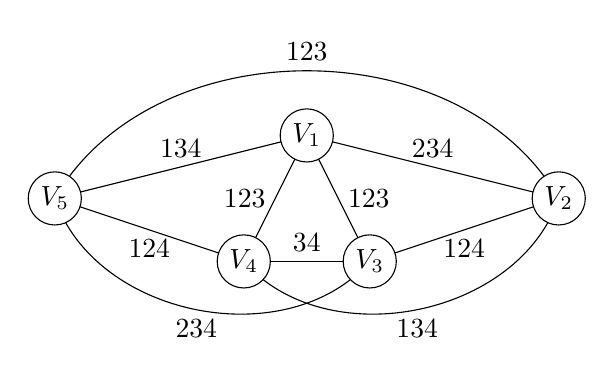
\begin{tikzpicture}[scale=0.8]
      \draw[bend right=60] (4, 0.5) to node[midway, above] {$123$} (-4, 0.5); 
      \draw (-4, 0.5) to node[midway, below] {$124$} (-1, -0.5); 
      \draw (-1, -0.5) to node[midway, above] {$34$} (1, -0.5); 
      \draw (1, -0.5) to node[midway, below] {$124$} (4, 0.5); 
      \draw (0, 1.5) to node[midway, above] {$234$} (4, 0.5); 
      \draw (0, 1.5) to node[midway, above] {$134$} (-4, 0.5); 
      \draw (0, 1.5) to node[midway, left] {$123$} (-1, -0.5); 
      \draw (0, 1.5) to node[midway, right] {$123$} (1, -0.5); 
      \draw[bend left=60] (4, 0.5) to node[midway, below] {$134$} (-1, -0.5); 
      \draw[bend right=60] (-4, 0.5) to node[midway, below] {$234$} (1, -0.5);
      
      \foreach [count=\i] \x/\y in {0/1.5, 4/0.5, 1/-0.5, -1/-0.5, -4/0.5} { 
        \fill[white] (\x, \y) circle (12pt);
        \draw (\x, \y) circle (12pt);
        \node at (\x, \y) [] {$V_{\i}$}; 
      }
    \end{tikzpicture}
    \caption{Example of an $(4, n, 5)$-blowup not containing a double $K_3$.}
    \label{fig:blowup}
  \end{figure}
\end{center}

\begin{definition}
  Let $f(m, n, r)$ denote the maximum of $e(G_1) + e(G_2) + \dots + e(G_m)$ such that $G_1, G_2, \dots, G_m$ is a double $K_r$-free $(m, n, N)$-blowup for some $N < R_{\binom{m}{2}}(r)$.
\end{definition}

This turns out to be exactly the construction which determines $\phi(m, n, F)$ when $F$ is a complete graph: 

\begin{theorem}\label{thm:blowup}
  For $m, n, r \geq 3$, 
  \[ 
    \phi(m, n, K_r) = f(m, n, r).
  \]
\end{theorem}

While computing $f(m, n, r)$ is a finite calculation, the Ramsey number $R_{\binom{m}{2}}(r)$ unfortunately appears to be intractable in general. It is known that $R_2(3) = 6$ and $R_3(3) = 17$ and $R_2(4) = 18$, but no further multicolor Ramsey numbers are known~\cite{ConlonFerber2021,Lefmann1987}. In the special case $r = m = 3$, the following holds: 

\begin{theorem}\label{thm:triangles}
  For $n \geq 1$,
  \[
    \phi(3, n, K_3) = \binom{n}{2} + \left\lfloor \frac{n^2}{2} \right\rfloor.
  \]
\end{theorem}

The same problem immediately becomes difficult when $m$ is increased by 1. The blowup construction in Figure \ref{fig:blowup} shows $\phi(4, n, K_3) - [\binom{n}{2} + 3\ex(n, K_3)] \geq n^2/100$ as $n \to \infty$. This suggests the actual values of $\phi(m, n, K_r)$ can be significantly larger than our trivial lower bound. We leave it as an open problem to determine $\phi(m, n, K_r)$ for $r, m \geq 3$ and $(r, m) \neq (3, 3)$.

\subsection{Definitions and Notations}

Denote the set of first $n$ positive integers as $[n] = \{1, 2, \ldots, n\}$. Given a set $X$, we denote $2^X$ as the power set of $X$. Let $G = (V, E)$ be a graph. Let $V(G)$ denote the vertex set and $E(G)$ denote the edge set of $G$. Let $e(G) = |E(G)|$ be the number of edges in $G$. For vertex $v \in V(G)$, we denote by $N_G(v) = \{u \in V(G) : \{u, v\} \in E(G)\}$ the neighborhood of $v$. Given two graphs $G_1, G_2$, we denote $G_1 \cup G_2$ as the graph on $V(G_1) \cup V(G_2)$ with edge set $E(G_1 \cap G_2) = E(G_1) \cup E(G_2)$. Similarly, we define $G_1 \cap G_2$ as the graph on $V(G_1) \cap V(G_2)$ with edge set $E(G_1 \cap G_2) = E(G_1) \cap E(G_2)$. In this thesis, we reserve $n$ to denote the number of vertices in a graph. We call a $n$-vertex complete graph $K_n$, and a complete bipartite graph $K_{a, b}$, where $a, b$ are the sizes of its parts. Given graph $G, H$, define $G + H$ as the graph fully connecting $G, H$, i.e. $V(G + H) = V(G) \cup V(H)$ and $E(G + H) = E(G) \cup E(H) \cup \{\{u, v\} : u \in V(G), v \in V(H)\}$. Given graphs $G$ and $F$, we say that $G$ is $F$-free if $G$ does not contain $F$ as a subgraph. We denote $\ex(n, F)$ to be the maximum possible number of edges an $F$-free graph on $n$ vertices, and we call a $F$-free graph achieving this maximum an extremal graph for $F$. Let $v$ be a vertex from $G_1, G_2, \ldots, G_m$. Unless otherwise specified, we denote $d(v)$ as the sum of the degree of $v$ over all $G_i$.